\chapter{Technical Documentation}
\label{chapter:technical_documentation}

The implementation of our autonomous racing agent relies on a complex set of libraries and tools. In this chapter, we will describe the libraries and tools we used and we will briefly explain how some of them work. We will also discuss our implementation the behavior of the autonomous racing agent. The installation instructions and instructions on how to deploy and use the software used and developed in this thesis are covered in the following chapter \ref{chapter:user_documentation}.

\section{Robot Operating System}

\gls{ROS} is an open-source set of libraries and tools built on top of Linux. Processes running under this operating system are referred to as nodes and they can be distributed across multiple computers connected over a wired or wireless network or through a serial port. Nodes can be programmed in many different programming languages but the most common and officially supported languages are Python and C++.

Nodes communicate between each other using a publisher/subscriber pattern. A node can advertise any number of topics through which it publishes its outputs in a form of messages. It can also subscribe to topics advertised by other nodes and it can work with the received messages as its outputs. This way it is possible to create a complex system by combining many small and simple specialized nodes.

Each topic has an assigned message type which defines the structure of the data. There is a large number of standard messages which are used by authors of public libraries. This way it is often possible to replace one library with a different one without additional changes to other nodes. This can be useful for example when one sensor is replaced by a device of the same type but from a different vendor whose \gls*{ROS} node publishes the same standard message type. Programmers can also define their custom message types which are better suited for their application.

\gls*{ROS} comes with a variety of tools for debugging and visualization of the data passed through the topics. One of these tools is \verb|Rviz|. It is a convenient way of visualizing the current state of the system. We use this tool to visualize the telemetry data from the vehicle on a laptop while it is driving along the racing circuit. The configuration we used during our experiments is included in the attached files as \verb|/ubuntu/mapping.rviz| and \verb|/ubuntu/race.rviz|.

We use the latest stable release of \gls*{ROS} at the time of writing this thesis named ``Melodic Morenia'' which is compatible with Ubuntu 18.04 LTS. Further information about \gls*{ROS} and tutorials which describe how to work with it are available on the official website of the \gls*{ROS} project\footnote{https://www.ros.org}.

\section{Architecture of the Distributed System}

The setup of our robot consists of the NVIDIA Jetson Nano board which is mounted on the vehicle, two Arduinos which are connected to the Jetson through a serial port, and a notebook which is connected to Jetson over Wi-Fi. Jetson acts as a \gls*{ROS} master machine, Arduinos act as an interface between Jetson and low-level hardware, and the notebook is used only to monitor telemetry data. The graph of this architecture and the connected sensors is depicted in Figure~\ref{fig:ros_diagram}.

\begin{figure}
	\centering
	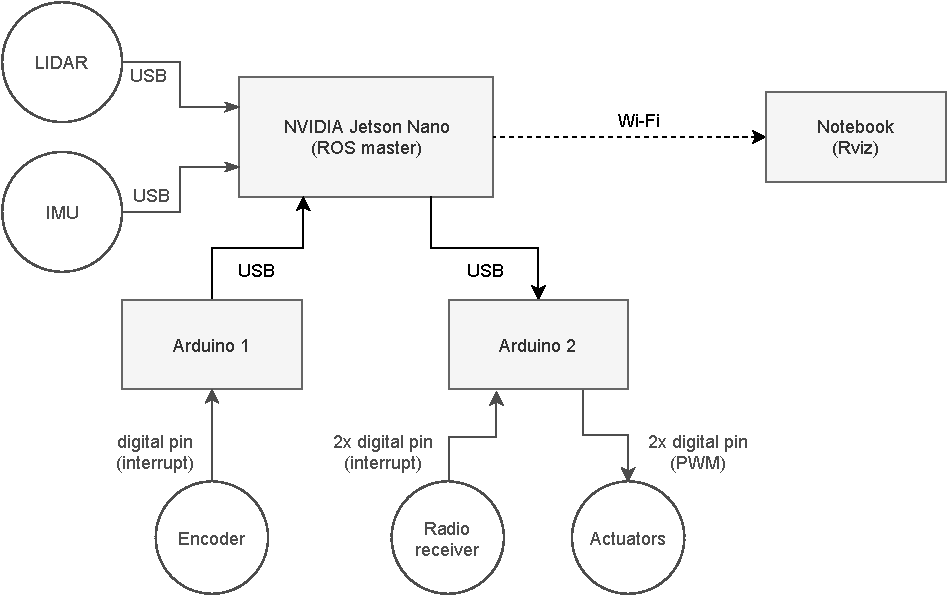
\includegraphics[width=125mm]{../img/ros_diagram}
	\caption{This figure shows how the computers and sensors which make up the experimental vehicle are connected with each other and the direction of data flow between the devices.}
	\label{fig:ros_diagram}
\end{figure}

The communication between the Arduinos and the Jetson takes place over over USB. This is possible thanks to the \verb|rosserial| package\footnote{http://wiki.ros.org/rosserial}. The Arduinos need to include the \verb|ros_lib| library which allows it to subscribe to topics and to publish messages. On Jetson, the communication on each serial port is handled by an instance of a \verb|rosserial_python| node.

\subsection{Coordinate Frames}

\Gls{ROS} includes a very useful way of keeping track of the relative position between different parts of the robot and the position of the robot itself on a map. The package which provides this functionality is called \verb|tf|\footnote{http://wiki.ros.org/tf}. \verb|tf| maintains a tree structure of coordinate frames and it keeps track of transformations between these coordinate frames as they change over time. The updates to the transformations are shared through a regular \gls*{ROS} topic called \verb|tf| of the \texttt{tf/tfMessage}\footnote{http://docs.ros.org/kinetic/api/tf/html/msg/tfMessage.html} type. The \verb|tf| package provides libraries for both Python and C++ which make accessing the current state of the whole system and manipulating with the linear transformations easy.

Our implementation adheres to the standard naming convention of coordinate frames as it is defined in \gls{REP} 105\footnote{https://www.ros.org/reps/rep-0105.html}. The vehicle has a \verb|base_link| frame attached to it. Each of the sensors has their own coordinate frame and there is a static transformation between the sensor and the base link using the \texttt{static\_\allowbreak transform\_\allowbreak publisher} node from the \verb|tf| package. The \gls*{IMU} gives us the current roll and pitch of the vehicle. We use the \texttt{hector\_imu\_attitude\_tf} node\footnote{https://github.com/tu-darmstadt-ros-pkg/hector\_slam/tree/catkin} to publish this transformation between \texttt{base\_link} and \texttt{base\_footprint}, which is the ``stabilized'' coordinate frame. The root (``fixed'') \verb|tf| frame is called \verb|map|. The transformation between the \verb|map| frame and the \verb|base_footprint| represents the pose of the vehicle on the map. This transformation is calculated and published through different nodes in the mapping and racing tasks and we will come back to it later.

\subsection{Sensors}

Each of the sensors connected through USB uses their own drivers for communication over the serial link. Luckily, open-source \gls*{ROS} packages for both the \gls*{LIDAR} and the \gls*{IMU} are available and both of them publish the data in the form of standard \verb|sensor_msgs/LaserScan|\footnote{http://docs.ros.org/melodic/api/sensor\_msgs/html/msg/LaserScan.html} and \verb|sensor_msgs/Imu|\footnote{http://docs.ros.org/melodic/api/sensor\_msgs/html/msg/Imu.html} messages. The data from the motor shaft encoder is published in the form of \verb|std_msgs/Float64| message and it contains the number of revolutions since the Arduino was last powered or reset. The source code for the Arduino is available in the attached source files in \verb|/controller-arduino/wheel_encoders/wheel_encoders.ino|.

The raw data we receive from the \gls*{LIDAR} and the \gls*{IMU} are not readily usable. We had to introduce a layer of preprocessing for both these sensors:

\begin{enumerate}
	\item The \gls*{LIDAR} is rigidly attached to the vehicle and so the laser scan is affected by the roll and pitch of the vehicle. We use \texttt{LaserScanBoxFilter} from the \texttt{laser\_filters} package\footnote{http://wiki.ros.org/laser\_filters} to remove points which are too close to the ground (the vehicle might see the ground when it is slowing down or braking) and which are too high above the ideal plane (the vehicle might see the ceiling or over the obstacles when it accelerates). The configuration for the \gls*{LIDAR} is stored in \texttt{/racer-jetson/\allowbreak catkin\_ws/\allowbreak src\allowbreak racer/\allowbreak launch/ydlidar.launch}.
	
	\item The coordinate frame of the \gls*{IMU} is not ideally aligned with the coordinate frame of the vehicle. Even though it should be possible, we were not able to get correct roll and pitch transformations using the \texttt{  static\_transform\_publisher} node of the \texttt{tf} package. To overcome this issue, we implemented a custom node in C++ called \verb|fix_imu| in the \verb|racer_sensors| package, which publishes the correct transformation. We also set positive values on the diagonals of covariance matrices to make the \gls*{IMU} message valid, because the \gls*{ROS} package for the IMU we use  \verb|bnp055_usb_stick|\footnote{https://github.com/yoshito-n-students/bno055\_usb\_stick} does not set them correctly. The configuration for the \gls*{IMU} is stored in \texttt{/racer-jetson/\allowbreak catkin\_ws/\allowbreak src\allowbreak racer/\allowbreak launch/imu.launch}.
\end{enumerate}

\section{Mapping}

In order to race, our vehicle needs a map of the racing track. The robot can create its own map using an algorithm called \gls{SLAM}. We use a library called Hector \gls*{SLAM} created by a team from the Technical University of Darmstadt.

To make things simple, we steer the vehicle manually using its remote controller. The robot collects data from the \gls*{LIDAR} as it moves along the track and it performs scan matching between the \gls*{LIDAR} scans and a 2D occupancy grid which it has built so far. For an already built part of the map and a \gls*{LIDAR} scan consisting of $n$ points, the task of the scan matching algorithm is to find a rigid body transformation $\xi =\left( p_x, p_y, \phi\right)$, which gives best alignment with the already built map. The authors formulate this problem as an optimization problem for solving in \cite{HectorSlam}:

$$
\xi^* = \underset{\xi}{\arg\min} \sum_{i=1}^n\left[ 1 - M\left( S_i\left( \xi\right)\right)\right]^2,
$$

where $S_i\left(\xi\right)$ are the world coordinates of scan point $s_i$ after applying the transform $\xi$ and the function $M$ gives the value of the occupancy grid at the given coordinates. After obtaining the transformation, the laser scan is aligned with the occupancy grid and each endpoint of a laser ray is marked as an obstacle into the occupancy grid.

Hector SLAM provides a \gls*{ROS} node \verb|hector_mapping| which subscribes to a topic providing \verb|sensor_msgs/LaserScan| messages and publishes its output in a topic of type \verb|nav_msgs/OccupancyGrid|\footnote{http://docs.ros.org/melodic/api/nav\_msgs/html/msg/OccupancyGrid.html}. The node also publishes a \verb|tf| transformation between the \verb|map| frame and the \verb|base_footprint| frame. An important parameter is the resolution of the occupancy grid which we chose to be \SI{5}{\centi\meter}. When the mapping is complete, the final map can be saved into a file using a \verb|map_saver| node from the \verb|map_server| package\footnote{http://wiki.ros.org/map\_server\#map\_saver}. We prepared a \gls*{ROS} launch file with the configuration of all nodes necessary for this task. This configuration is included in the attached files in \texttt{/racer-jetson/\allowbreak catkin\_ws/\allowbreak  src/\allowbreak  racer/\allowbreak  launch/create\_map.launch}. The proper usage of this launch file is described in Chapter~\ref{chapter:user_documentation}.

\section{Racing}

Racing is the most important and the most complicated part of the implementation. It can be split into three groups of \gls*{ROS} nodes: odometry and localization, agent behavior, and a hardware interface. We prepared a \gls*{ROS} launch file with the configuration of all nodes necessary for the racing task in the attached files in \newline\verb|/racer-jetson/catkin_ws/src/racer/launch/race.launch|. This launch file requires two arguments: a map definition file and a circuit definition file. The proper usage of this launch file is described in Chapter~\ref{chapter:user_documentation}.

\subsection{Map}

We use \verb|map_server| node of the \verb|map_server| package to serve the previously recorded occupancy grid to the other nodes. The map is stored in two files: a \verb|.yaml| file with map metadata and a \verb|.pgm| file with the occupancy grid stored as a bitmap. It is necessary that the \verb|.yaml| configuration file contains a correct relative path to the bitmap file. The map server publishes a topic called \verb|map| of type \verb|nav_msgs/OccupancyGrid|. This node also provides a service for one-time retrieving the map without subscribing to the topic.

\subsubsection{Costmap} In order to prevent collisions, we use a \gls*{ROS} package \verb|costmap_2d|\footnote{http://wiki.ros.org/costmap\_2d} to inflate the areas around obstacles according to a bounding rectangle around the vehicle. The result of this node is another \verb|nav_msgs/OccupancyGrid| topic with cell values marking the ``cost'' of each cell instead of the regular ternary status (free/obstacle/unknown). The higher the cell cost is, the closer the cell is to an obstacle. Values above certain threshold value are considered ``lethal'' and if the center of the vehicle were in this position it would be colliding with an obstacle. Collision detection is then just a matter of a single query into the occupancy grid to check if the cell which contains the center point of the vehicle.

This \verb|costmap_2d| can also work directly with the laser scan from the LIDAR and overlay it with the map using the latest \verb|tf| transformation between the \verb|map| and \verb|lidar| coordinate frames and mark obstacles which were not present during mapping into the resulting occupancy grid. Unfortunately, this feature was flaky and we had to disable it in the final version of our configuration. The laser frame would often be misaligned with the original map for a brief moment and it would mark certain areas of free space as obstacles. The ``clearing'' feature, which is supposed to remove obstacles from the costmap based on new laser scans, did not work properly and the map soon became filled with ghost obstacles.

\subsection{Odometry and Localization}

Odometry is an estimate of how position of the robot changes over time based on data from sensors which measure the movement of the robot. Odometry is supposed to be continuous and there should not be any sudden changes in the position of the vehicle.

Our vehicle has two sources of odometry: the number of revolutions of the motor shaft and the accelerations measured by the IMU. We implemented a simple \gls*{ROS} node called \verb|odometry_node| in C++ which subscribes to the motor shaft encoder and the steering commands supplied to the vehicle. From the number of revolutions and an assumption that the wheels are not skidding we can estimate the distance the vehicle travelled since the last update. From the steering command, we can estimate the steering angle of the front wheels of the vehicle. From these two inputs, we can estimate how the vehicle body translated and rotated using a simple kinematic vehicle model. This approach was inspired by the MIT RACECAR VESC odometry \gls*{ROS} node\footnote{https://github.com/mit-racecar/vesc}. Source code of the odometry node is located in the attachments in \verb|/racer-jetson/catkin\_ws/src/odometry|.

The data from the odometry node and the \gls*{IMU} are then fused into a single estimate using the \verb|robot_pose_ekf| node\footnote{https://wiki.ros.org/robot\_pose\_ekf}. This node uses \gls*{EKF} to estimate the most likely location from the input sources and their covariances. This node produces a \verb|tf| transform between the \verb|odom| and \verb|base_footprint| frames. We also tried to use a newer \gls*{ROS} package \verb|robot_localization| which also implements an \gls*{EKF}, but the results were less accurate.

The data from the odometry sensors is inherently noisy and inaccurate and the estimated position of the robot will become more and more inaccurate over time. This phenomenon is referred to as drift. To counteract the drift, we perform a correction using the \gls*{AMCL} algorithm. This algorithm uses the data from the \gls*{LIDAR} to determine the position of the vehicle in the map based on the distances to the obstacles around it. Unlike odometry, the sequence of position updates is not expected to be continuous and the resulting location can in theory be a point anywhere on the map. We use an implementation of this algorithm in the \verb|amcl| \gls*{ROS} package\footnote{http://wiki.ros.org/amcl}. The \verb|amcl| node from this package publishes a \verb|tf| transformation between \verb|map| and \verb|odom| to correct the odometry drift. The \verb|tf| tree is captured in Figure~\ref{fig:tf_tree_racing}.

\begin{figure}
	\centering
	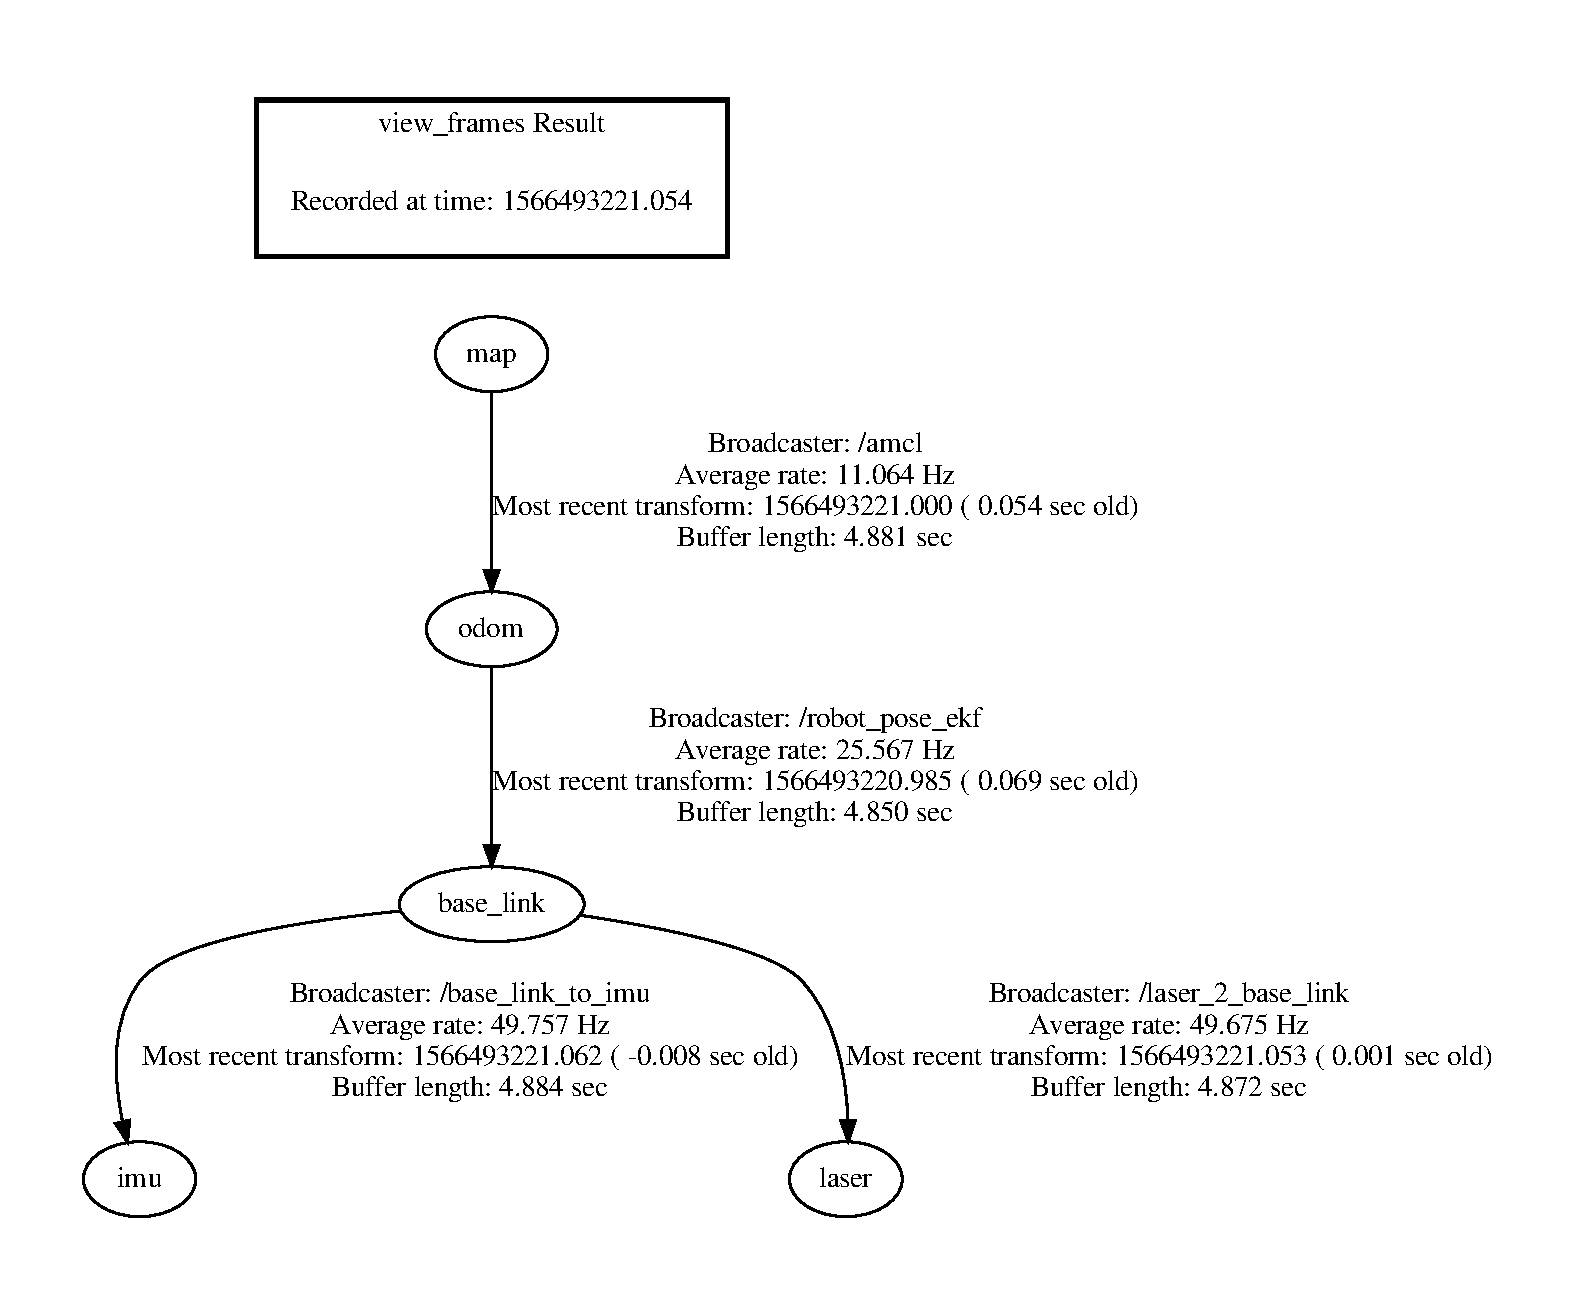
\includegraphics[width=125mm]{../img/racing_tf_tree}
	\cprotect\caption{The tree shows which nodes publish transformations between the coordinate frames and at what average rate the transformations are updated. This diagram is the output of the \verb|tf| \verb|view_frames| diagnostics tool.}
	\label{fig:tf_tree_racing}
\end{figure}

% \todo[inline]{Update the figure with a one with base_footprint}

Tuning odometry and localization ROS libraries to obtain reliable data at high rates proved to be difficult. In some scenarios, the robot would ``get lost'' when the localization algorithm would match the scan incorrectly and it would report incorrect location of the robot on the map. This can easily lead into a crash of the robot with a wall or an obstacle. The \gls*{AMCL} algorithm will sometimes manage to find the correct location after a few seconds, but in these cases it was necessary to take over control over the vehicle manually with a remote control and stop the vehicle until the robot corrects its location. The \gls*{AMCL} \gls*{ROS} node has many parameters which we spend many hours tuning them in order to get the best possible results. The final configuration is available in \newline\verb|/racer-jetson/catkin_ws/src/racer/launch/amcl_localization.launch|.

\subsection{Agent Behavior}
\label{sec:agent_impl}

We implemented the individual components of the behavior of the agent, as it was described in Chapter~\ref{chapter:agent} and visualized in Figure~\ref{fig:racing_agent_diagram}, with four \gls*{ROS} nodes as part of the \verb|racer| package we implemented:

\begin{enumerate}
	\item \verb|current_state_node|,	
	\item \verb|circuit_node|,
	\item \verb|planning_node|,	
	\item \verb|dwa_planning_node|.
\end{enumerate}

The C++17 implementation of the \verb|racer| package is located in \texttt{/racer-jetson/\allowbreak catkin\_ws/\allowbreak src/racer/} and it contains the source code of the individual \gls*{ROS} nodes as well as the source code of the algorithms which were described in this thesis. The definitions of the messages are located in a separate package \texttt{/racer-jetson/\allowbreak catkin\_ws/\allowbreak src/racer\_msgs/}. All of the coordinates used by \verb|racer| package nodes are in the global \verb|map| coordinate frame unless stated otherwise.

\subsubsection{Current State Node}

This node listens to the \verb|tf| transformations and converts them into a custom message format \verb|racer_msgs/State|. This message contains the 2D position of the vehicle, its orientation, and its immediate speed in the heading direction in the \verb|map| \verb|tf| coordinate frame.

To achieve the highest possible update rate, we had to manually combine the latest odometry estimate \verb|odom -> base_link| and the latest odometry drift correction \verb|map -> odom| by multiplying their transformation matrices. When we tried obtaining the transformation \verb|map -> base_link| from the \verb|tf| library directly, the update rate was the same as the transform published by \gls*{AMCL}. By manually combining the transformations, we would be able to publish the current state estimate in sync with odometry updates.

If we assume that the fused odometry gives us reasonable movement estimates over short time periods and that we use a very recent drift correction, this workaround is reasonable. The maximum rate at which we can control the actuators is \SI{50}{\hertz} and we are able to achieve vehicle state updates at the rate of \SI{25}{\hertz} (see Figure~\ref{fig:tf_tree_racing}).

\subsubsection{Circuit Node}

The circuit node analyzes the occupancy grid of the current track based on a circuit definition for the track at the start of the race using Algorithm~\ref{alg:find_apexes}. The circuit definition is a list of checkpoints on the map. The vehicle is supposed to drive along the track in a way such that it passes these checkpoints in the given order. The starting position is considered to be an implicit checkpoint. This list is loaded from a \verb|.yaml| configuration file which contains an array of 2D~point coordinates under the key \verb|check_points|. The coordinates are strings with the $x$ and $y$ coordinate separated by a whitespace. An example of such configuration file with two would look like this:

\begin{verbatim}
check_points:
  - "6.385 -0.521"
  - "-0.639 -4.226"
\end{verbatim} 

Later during the race, this node monitors the state of the vehicle and it produces a list of the next waypoitns in a custom message format
\texttt{racer\_msgs/\allowbreak Waypoints}. The number of waypoints which are published can be configured using the \texttt{lookahead} parameter of the node.

\subsubsection{Planning Node}

The planning node plans a trajectory based on the last known state of the vehicle through the list of next waypoints and publishes it in the form of a custom message type \verb|racer_msgs/Trajectory|. The planning node uses the SEHS algorithm we described in this thesis because it is more efficient than Hybrid~A*. The source code of the node can be easily modify to switch to Hybrid~A* if necessary.

This node will try to re-plan the trajectory as often as possible, but it is limited by a maximum updated frequency which is configurable. This is necessary because sometimes the vehicle passes close to an obstacle while following the last published trajectory and the localization algorithm briefly fails and determines the location of the vehicle in a way that the planning node detects an collision right in the initial state. The localization algorithm will recover with a new measurement of the sensors, but in the meantime, the planning algorithm could report tens or hundreds of failures because of the incorrect location. By limiting the maximum update frequency for example to \SI{2}{\hertz} we will still get frequent updates of the trajectory and the node will be more stable.

Most of the time during a race, the vehicle drives forward. and it does not come to a full stop or even require driving in reverse. Therefore, we prefer planning just with actions for driving forward only. If it is not possible to find a trajectory like this, we will try again now also with actions which allow driving in reverse. This way we can generate trajectories faster than if we always allowed going in reverse most of the time by limiting the number of actions and therefore we decrease the size of the nodes we open.

\subsubsection{Following Node}

This node finds the best control input for the actuators in order to follow the planned trajectory based on the current state of the vehicle using the \gls{DWA} algorithm. \gls*{DWA} has a set of actions it chooses from. The algorithm simulates how the state of the vehicle would change if a given action was used for a given period of time and then it selects the one, which allows it to track the reference trajectory better than the others. We give the algorithm many different actions including actions for driving in reverse.

The node publishes a standard message type \verb|geometry_msgs/Twist|\footnote{http://docs.ros.org/melodic/api/geometry\_msgs/html/msg/Twist.html}. By using this message type, we mimic the output of the open source \verb|move_base| \gls*{ROS} package\footnote{http://wiki.ros.org/move\_base}. The throttle level is stored in the \verb|linear.x| component ant the steering level is stored in \verb|angular.z|. This message is later translated into a \gls*{PWM} signal for the actuators by the hardware interface component.

There is an alternative following node which implements the Pure Pursuit algorithm for steering and \gls*{PID} controller for regulating the speed. This node is called \verb|geometric_following_node| and it listens to and publishes the same topics as the \verb|dwa_following_node|. We included this node even though it is not used by default because it does not have the ability to avoid previously unknown obstacles and it does not support going in reverse. Both of the algorithms simple yet interesting and the node can be useful in certain scenarios.

\subsection{Hardware Interface}

The \verb|Arduino 2| from Figure~\ref{fig:rosdiagram} has two responsibilities:

\begin{enumerate}[label=(\roman*)]
	\item subscribe to the commands produced by the agent and transform them into electrical signals for the servo and the \gls*{DC} motor,
	\item monitor the input from the radio controller and in case that there is a strong signal, disable the autonomous mode and forward the signal to the actuators to allow the human supervisor to control the vehicle directly.
\end{enumerate}

The implementation of the behavior for \verb|Arduino 2| is included in the attached \verb|*.ino| files in \verb|/controller-arduino/steering_node/|.

\subsubsection{Conversion of Commands to PWM}

The agent behavior produces actions in the form of two real numbers between $-1$ and $1$ for the steering angle and for the throttle level. These numbers are mapped to \gls*{PWM} duty cycles which are then passed to the actuators through PWM-capable digital pins of the Arduino.

The mapping for the steering servo is straightforward. The $\interval{-1}{1}$ interval is directly mapped to the interval of $\interval{\SI{1200}{\micro\second}}{\SI{1800}{\micro\second}}$ which are the bounds of the servo of our vehicle. The wheels steer to the leftmost position when the duty cycle is set to \SI{1200}{\micro\second}, at \SI{1500}{\micro\second} the wheels are aligned with the body of the vehicle, and at \SI{1800}{\micro\second} the wheels are in the rightmost position.

The mapping of the signal for the \gls*{DC} motor is a bit more complicated. The range of duty cycles $\interval{\SI{1400}{\micro\second}}{\SI{1600}{\micro\second}}$ does not produce enough torque to set the vehicle into motion. The range of $\interval{\SI{1000}{\micro\second}}{\SI{1400}{\micro\second}}$ corresponds to reversing, where at \SI{1000}{\micro\second} the motor spins the fastest in the reversing direction. The range of $\interval{\SI{1600}{\micro\second}} {\SI{2000}{\micro\second}}$ corresponds to going forward, where at \SI{2000}{\micro\second} duty cycle the motor spins the fastest in the forward direction. The boundary values of \SI{1400}{\micro\second} and \SI{1600}{\micro\second} are not fixed and they vary based on how much is the battery charged. We therefore use the following mapping:

\[
	\begin{dcases}
		\interval{-1}{-0.05} & \rightarrow \interval{\SI{1000}{\micro\second}}{\SI{1400}{\micro\second}} \\
		\interval{-0.05}{0.05} & \rightarrow \SI{1500}{\micro\second} \\
		\interval{0.05}{1} & \rightarrow \interval{\SI{1600}{\micro\second}}{ \SI{2000}{\micro\second}}
	\end{dcases}
\]

The limits can be adjusted for different needs, e.g. the maximum speed can be limited by lowering the maximum duty cycle.

\subsubsection{Manual Override}

The two signals from the radio receiver are connected to two interrupt pins of the Arduino. By measuring the time difference between the detection of a raising edge and a falling edge of the signal we can determine the width of the duty input cycle. If one of the two signals falls out of the range of $\interval{\SI{1400}{\micro\second}}{\SI{1600}{\micro\second}}$, we consider it to be the supervisors intervention and we will start forwarding the \gls*{PWM} signal directly to the actuators and we will stop processing the commands from the agent. The autonomous mode can be restored by physically pressing the reset button on the board.